\chapter{Results\label{cha:chapter6}}
\section{Data Acquisition}
The data acquisition was performed with 27 subjects in total, 12 (44\%) females and 15 (56\%) males. Participants had an average age of 26.4 years (17, 53, 6.39) and all 27 were right-handed (100\%). 19 (70\%) were students, 8 (30\%) had other occupations. All 27 (100\%) were right handed.
18 (66\%) subjects stated that their most used input modality is the their thumb while 4 (14\%) preferred using their index finger and 5(18\%) use both thumbs during interactions.\\

\begin{figure}[h!]
  \centering
  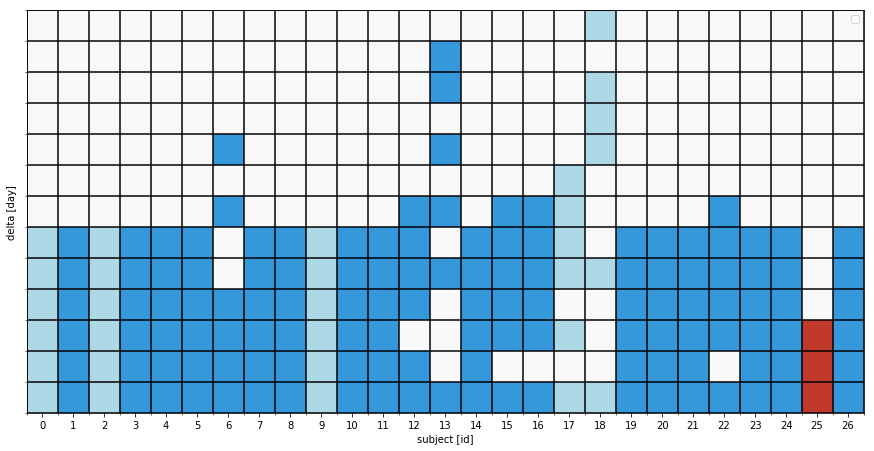
\includegraphics[width=1\textwidth]{participation_push.png}
  \caption{The figure shows on which days the participants took part in the field study. Light blue subjects which did not receive push notifications while subjects with dark blue marks had received push notifications. Red rectangles indicates a dropped out subject.} \label{fig:participation}
\end{figure}

In regards to the participation during the study, 26 subjects managed to finish all laboratory and field study trials while 1 subject dropped out in the field study. Figure \ref{fig:participation} shows on which day individual participants performed trails. 4 participants did not accept push notification and were therefore not reminded on a daily basis.

In total over 46.000 taps were generated in the whole data acquisition phase. To be more precise, approx. 25.000 taps were collected on the 5x4 grid, over 15.000 taps on the 4x3 grid and more than 5.000 taps on the 2x2 grid.

The devices used to obtain the tap information were 12 (45\%) Apple iPhone 6s, 10 (37\%) iPhone 6 and the least common device was the iPhone 7 with 5 (18\%).

\section{Laboratory and Field Comparison}
In this section, I present the classification results for the data acquired. The training data has been filtered based on the environment and the mobile device. After performing a grid search of the hyperparameter space for the SVM and the ANN, a 10-fold cross validation has been performed on the best estimator.

\subsubsection{2x2 Grid}
As illustrated in the box plot, for the 2x2 grid the results show that all classification accuracies are above guessing probability of $\frac{1}{4} = 25\%$ with the iPhone 7 performing best with a mean accuracy score of 0.87 (+/- 0.06) in the laboratory environment.

\begin{table}[h!]
  \centering
\begin{tabular}{|l|l|c|c|c|c|c|}
  \cline{3-7}
  \multicolumn{2}{c}{} & \multicolumn{4}{|c|}{\textbf{Accuracy}} & \textbf{Kappa} \\
  \hline
  \textbf{Device} & \textbf{Environment} & mean &   min &   max  & std &  mean \\
  \hline
  iPhone 6 & Lab &      0.76 &     0.68 &     0.85 &     0.06 &        0.68 \\
  & Field &      0.73 &     0.64 &     0.86 &     0.07 &        0.64 \\
  \hline
iPhone 7 & Lab &      0.87 &     0.73 &     0.96 &     0.06 &        0.83 \\
  & Field &      0.75 &     0.54 &     0.83 &     0.10 &        0.66 \\
  \hline
iPhone 6s & Lab &      0.86 &     0.80 &     0.94 &     0.05 &        0.81 \\
  & Field &      0.72 &     0.49 &     0.87 &     0.11 &        0.63 \\
  \hline
\end{tabular}
  \caption{Classification results for the 2x2 tapping grid.}
\end{table}

Results show that the model trained with data from the iPhone 7 outperform the models trained with the iPhone 6 and iPhone 6s, respectively. The iPhone 6 models shows least accuracy scores of 0.76 (+/- 0.06) for the controlled and 0.73 (+/- 0.07) for the uncontrolled environment.

% For the comparison of devices, the results yield that the iPhone 7 scores higher accuracies compared to the iPhone 6 and and the iPhone 6s for both environments. The iPhone 6 scores lowest with a mean accuracy of 0.76 (+/- 0.85) while the iPhone 7 performs best with a mean accuracy of 0.87 (+/- 0.96) in the controlled environment. For the field environnement the iPhone 7 scores a mean accuracy of 0.75 (+/- 0.83) while the iPhone 6 shows 0.73 (+/- 0.86).

Moreover, the results reveal that all mean accuracy scores across all devices are lower in the field compared to the laboratory environment. The fact that the classification results for both environments differ is confirmed by a Wilcoxon signed-rank test yielding that the fold accuracies in the laboratory were significantly higher than the fold accuracies in the field environment $Z = 24, p < 0.05$.

\begin{figure}[h!]
  \centering
  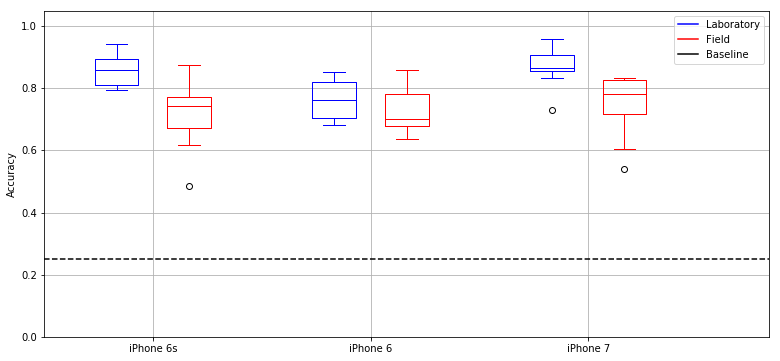
\includegraphics[width=1\textwidth]{results/lab-vs-field-2x2.png}
  \caption{The figure shows the tap inference accuracies for the 2x2 grid of the 10-fold cross-validation.} \label{fig:participation}
\end{figure}

\subsubsection{4x3 Grid}

As for the smallest of the three grids, similar results could be found showing that all inference accuracies are above the probability baseline of guessing which is $\frac{1}{12}= 8.33\%$ for the 4x3 grid. Similarly, the iPhone 7 scores best with a mean accuracy of 0.62 (+/- 0.10) in the laboratory environment.

\begin{table}[h!]
  \centering
\begin{tabular}{|l|l|c|c|c|c|c|}
  \cline{3-7}
  \multicolumn{2}{c}{} & \multicolumn{4}{|c|}{\textbf{Accuracy}} & \textbf{Kappa} \\
  \hline
  \textbf{Device} & \textbf{Environment} & mean &   min &   max  & std &  mean \\
  \hline
  iPhone 6 & Lab &      0.47 &     0.36 &     0.56 &     0.06 &        0.42 \\
  & Field &      0.41 &     0.35 &     0.48 &     0.04 &        0.35 \\
  \hline
iPhone 7 & Lab &      0.62 &     0.41 &     0.78 &     0.10 &        0.59 \\
  & Field &      0.48 &     0.31 &     0.63 &     0.10 &        0.43 \\
  \hline
iPhone 6s & Lab &      0.56 &     0.47 &     0.65 &     0.06 &        0.52 \\
  & Field &      0.42 &     0.29 &     0.54 &     0.07 &        0.36 \\
  \hline
\end{tabular}
  \caption{Classification results for the 4x3 tapping grid.}
\end{table}

Furthermore, the results show that the iPhone 7 models perform best, followed by the models trained on the iPhone 6s and iPhone 6, consecutively. Again, the iPhone 6 performs worst in comparison to the other devices yielding accuracies of 0.47 (+/- 0.06) in the controlled and 0.41 (+/- 0.04) in the uncontrolled environment. 

The Wilcoxon signed-rank test shows that the classification results for both environments differ significantly. The fold accuracies in the laboratory were statistically higher than the fold accuracies in the field environment $Z = 21, p < 0.05$.

\begin{figure}[h!]
  \centering
  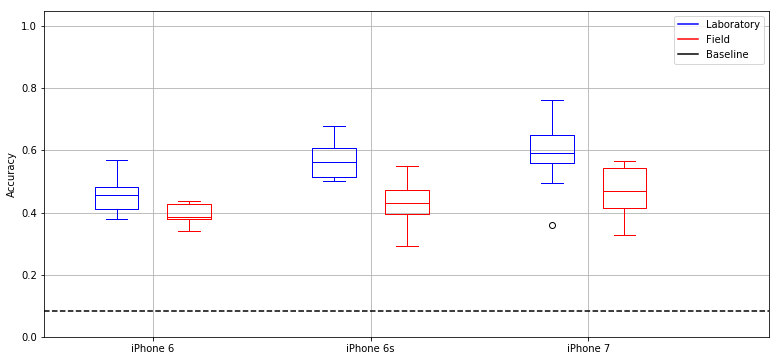
\includegraphics[width=1\textwidth]{results/lab-vs-field-4x3.png}
  \caption{The figure shows the tap inference accuracies for the 4x3 grid of the 10-fold cross-validation.} \label{fig:participation}
\end{figure}

\subsubsection{5x4 Grid}
For the grid with 20 distinguishable buttons the inference accuracies range from 0.46 (+/- 0.11) on the iPhone 7 to 0.28 (+- 0.03) on the iPhone 6. Results show that all inference accuracies are above the baseline of $\frac{1}{20} = 5\%$ for this classification problem.

\begin{table}[h!]
  \centering
\begin{tabular}{|l|l|c|c|c|c|c|}
  \cline{3-7}
  \multicolumn{2}{c}{} & \multicolumn{4}{|c|}{\textbf{Accuracy}} & \textbf{Kappa} \\
  \hline
  \textbf{Device} & \textbf{Environment} & mean &   min &   max  & std &  mean \\
  \hline
  iPhone 6 & Lab &      0.35 &     0.28 &     0.45 &     0.06 &        0.32 \\
  & Field &      0.28 &     0.23 &     0.33 &     0.03 &        0.24 \\
  \hline
iPhone 7 & Lab &      0.46 &     0.21 &     0.63 &     0.11 &        0.43 \\
  & Field &      0.34 &     0.25 &     0.47 &     0.08 &        0.31 \\
  \hline
iPhone 6s & Lab &      0.42 &     0.34 &     0.50 &     0.05 &        0.39 \\
  & Field &      0.30 &     0.18 &     0.38 &     0.06 &        0.26 \\
  \hline
\end{tabular}
  \caption{Classification results for the 5x4 tapping grid.}
\end{table}

Aligning with the results from the two previous grids, the iPhone 7 models show higher mean accuracies compared to the other devices. 

Furthermore, The Wilcoxon signed-rank test shows that the classification results for both environments alter significantly. The fold accuracies in the laboratory were significantly higher than the fold accuracies in the field environment $Z = 22, p < 0.05$.

\begin{figure}[h!]
  \centering
  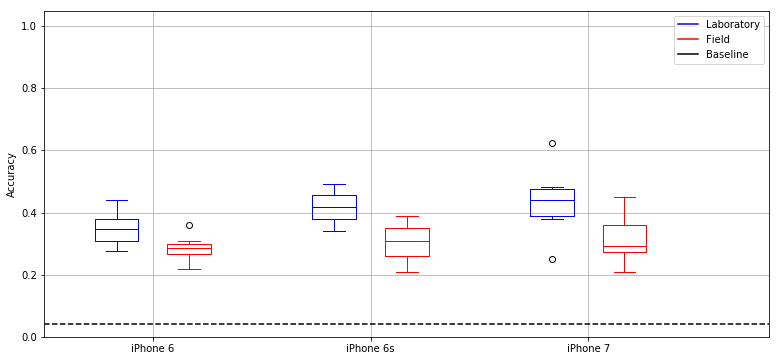
\includegraphics[width=1\textwidth]{results/lab-vs-field-5x4.png}
  \caption{The figure shows the tap inference accuracies for the 4x3 grid of the 10-fold cross-validation.} \label{fig:participation}
\end{figure}

\section{Input Modalities Comparison}
As for the comparison between environments, the same classification experiment was performed to detect differences in the predictive models between the two input modalities: Index finger and thumb. As the results between individual grid sizes are similar, only the 5x4 grid is represented here. Results for the other grids are to be found in the appendix.

The results show that across all devices the mean accuracy for thumb tap data was lower compared to data containing index finger taps. For the iPhone 7 a mean accuracy of 0.57 (+/- 0.05) was achieved for index taps compared to 0.35 (+/- 0.07) for thumb taps. A Wilcoxon signed-rank test shows that the classification results for both input modalities differ significantly. The fold accuracies for the thumb were statistically lower than the fold accuracies for the index finger Z = 2, p < 0.05.


\begin{figure}[h!]
  \centering
  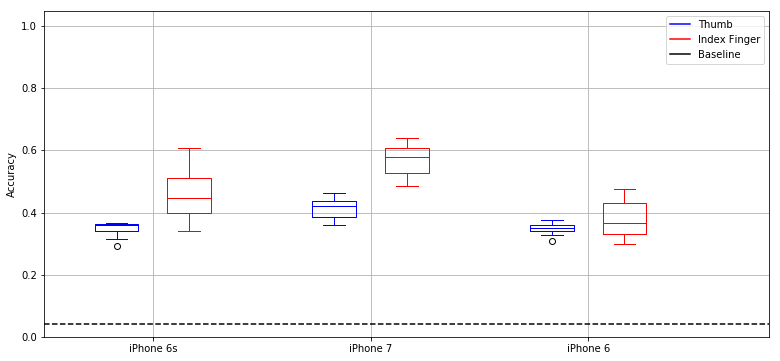
\includegraphics[width=1\textwidth]{results/index-vs-thumb-5x4.png}
  \caption{The figure shows the tap inference accuracies for the 5x4 grid of the 10-fold cross-validation.} \label{fig:participation}
\end{figure}

\begin{table}[h!]
  \centering
\begin{tabular}{|l|l|c|c|c|c|c|}
  \cline{3-7}
  \multicolumn{2}{c}{} & \multicolumn{4}{|c|}{\textbf{Accuracy}} & \textbf{Kappa} \\
  \hline
  \textbf{Device} & \textbf{Environment} & mean &   min &   max  & std &  mean \\
  \hline
  iPhone 6 & Index &      0.37 &     0.27 &     0.46 &     0.06 &        0.34 \\
  & Thumb &      0.31 &     0.24 &     0.39 &     0.04 &        0.27 \\
  \hline
iPhone 7 & Index &      0.57 &     0.48 &     0.63 &     0.05 &        0.55 \\
  & Thumb &      0.35 &     0.22 &     0.46 &     0.07 &        0.32 \\
  \hline
iPhone 6s & Index &      0.47 &     0.34 &     0.58 &     0.07 &        0.44 \\
  & Thumb &      0.33 &     0.21 &     0.46 &     0.07 &        0.29 \\
  \hline
\end{tabular}
  \caption{Classification results for the 5x4 tapping grid.}
\end{table}

\section{Body Posture Comparison}



\section{Discussion}
